\documentclass[10.5pt]{article}

\usepackage[english]{babel}
\usepackage[letterpaper,top=2cm,bottom=2cm,left=3cm,right=3cm,marginparwidth=1.75cm]{geometry}

% Packages
\usepackage{graphicx}
\usepackage{listings}
\usepackage{color}
\usepackage{dirtree}
\usepackage{amsmath}
\usepackage{geometry}
\usepackage{subcaption}
\usepackage{fancyhdr}
\usepackage{titlesec}

\usepackage{etoolbox}
\patchcmd{\thebibliography}{\section*{\refname}}{}{}{}

\pagestyle{fancy}
\fancyhf{}
\fancyhead[L]{Mystic Mayhem}
\fancyhead[R]{Saksham Khandelwal}
\fancyfoot[C]{\thepage}

\usepackage[colorlinks=true, allcolors=blue]{hyperref}

% Code styling
\definecolor{codegray}{gray}{0.9}
\lstset{
    backgroundcolor=\color{codegray},
    basicstyle=\ttfamily\small,
    breaklines=true,
    frame=single
}

% Title Page
\title{\Huge\textbf{Mystic Mayhem} \\ \Large{1v1 Angry Birds on Pygame} \\ \vspace{0.5cm} \large Project Report}
\author{Saksham Khandelwal \\ 24B0965 \\ CS108: SSL}
\date{\today}

\begin{document}
\thispagestyle{empty}
\maketitle

\tableofcontents
\newpage

\section{Abstract}
This project presents a turn based 1v1 game inspired by Angry Birds having a twist of wizard and spells, developed using Python and the Pygame library. Players take alternate turns to launch explodable projectiles at each other's towers which are subjected to gravity and drag, having a collision effect with the tower blocks. The objective is to strategically and precisely throw the spell orbs to destroy the opponent's tower. The game includes different pages for different actions, such as the player selection screen, main game world, leader board, and so on, and contains animations and background music to enhance the gaming experience. This project demonstrates the use of Python and its powerful game development library Pygame with integration of game design and physics implementations to offer engaging and competitive game play. \\

\section{Introduction}

The motivation behind this project came from my interest in exploring game development. While working on this, I wanted to create a unique gaming experience that blends strategy and fun, something that could be engaging and visually appealing. I decided to go with somewhat different theme of the game, mechanics inspired by \textit{Angry Birds}, but with a twist. I replaced the traditional slingshot and birds with wizards and magic orbs. This added a layer of creativity, allowing me to experiment with both visual style and gameplay mechanics.

The game is set in a mystical wizarding realm where arcane magic and elemental forces dictate the outcome of fierce one on one duels. Each player assumes the role of a powerful wizard standing atop a customized tower composed of enchanted blocks. These towers serve not only as visual symbols of each player's domain, but also as destructible structures that determine the victor. The goal is to demolish the opponent’s tower by launching spell orbs that behave under simulated physics including gravity, drag, collision response, and optional mid air explosion.

The core mechanic is turn based: players alternate launching their orbs by clicking and dragging in the desired direction. Strategy is vital, as the player must take into account angle, force, and timing. The spell system currently includes basic orb types but is designed for extensibility with more complex spells and effects in future iterations.

Overall, this project serves as an exploration of applying fundamental programming and design concepts such as event handling, physics simulation, asset management, and user interface design into the construction of a cohesive and enjoyable 2D game using Python and Pygame.

\section{Project Architecture}
\subsection{Tools and Libraries}
The module used are:
\begin{itemize}
        \item \texttt{pygame-ce} - It is the community maintained fork of the original Pygame library, offering features for building games and multimedia applications.
        \item \texttt{os} - It lets Python interact with the operating system, including file paths and was used to load assets with correct path handling.
        \item \texttt{random} - It provides functions to generate random numbers and choices. It was used to create randomized ball types, tower structures, or gameplay variations to increase replayability.
        \item \texttt{math} - This module provides basic mathematical functions and constants. It was mostly used for trigonometric calculations and motion physics.
        \item \texttt{numpy} - It is a powerful library for numerical computing and array operations. It was used for vector based physics calculations and handling numerical arrays efficiently.
    \end{itemize}

\newpage

\subsection{Directory Structure}\label{sec:directory-structure}
    The project directory is as follows:

    \dirtree{%
        .1  ..
        .2 states.
        .3 credits.py.
        .3 end\_game.py.
        .3 game\_world.py.
        .3 leaderboard.py.
        .3 loading.py.
        .3 main.py.
        .3 options.py.
        .3 pause\_menu.py.
        .3 select.py.
        .3 state.py.
        .3 tutorial.py.
        .2 assets.
        .3 fonts.
        .3 sprites.
        .3 sound.
        .2 game.py.
        .2 leaderboard.txt.
        .2 options.txt.
    }

    \begin{itemize}
        \item \textbf{game.py} - The main game loop loading assets and calling last state update and render functions.
        \item \textbf{states} - Contains different python files for different states
        \item \textbf{assets} - Contains all the images, sounds, and fonts used in the game.
        \item \textbf{leaderboard.txt} - Contains the wins and losses of each player along with their ranking
        \item \textbf{options.txt} - Contains the audio and resolution settings to apply them at start of game.
    \end{itemize}
    
\vspace{1cm}
\section{Game Instructions and Gameplay}
\subsection{Instructions to Run the Game}
Make sure python is installed on your system along with all modules mentioned above. \\ \\
Also ensure that \texttt{pygame-ce} and only \texttt{pygame-ce} are only installed, not the traditional pygame.
    If you have the traditional pygame installed, run: \\
    \texttt{pip uninstall pygame} \\
    \texttt{pip install pygame-ce} \\ \\
The game can be launched by using the suitable command of the following two in terminal opened in the directory containing game.py: \\
    \texttt{python game.py} \\
    \texttt{python3 game.py} \\

\newpage

\subsection{Gameplay}
\subsubsection{Loading and Intro Screen}
The game starts with the loading screen during which all assets used during the game are loaded at once and then intro screen is showed from which you can proceed by pressing the Enter key
\vspace{0.3cm}
\begin{figure}[h!]
    \centering
    \begin{minipage}[t]{0.45\textwidth}
        \centering
        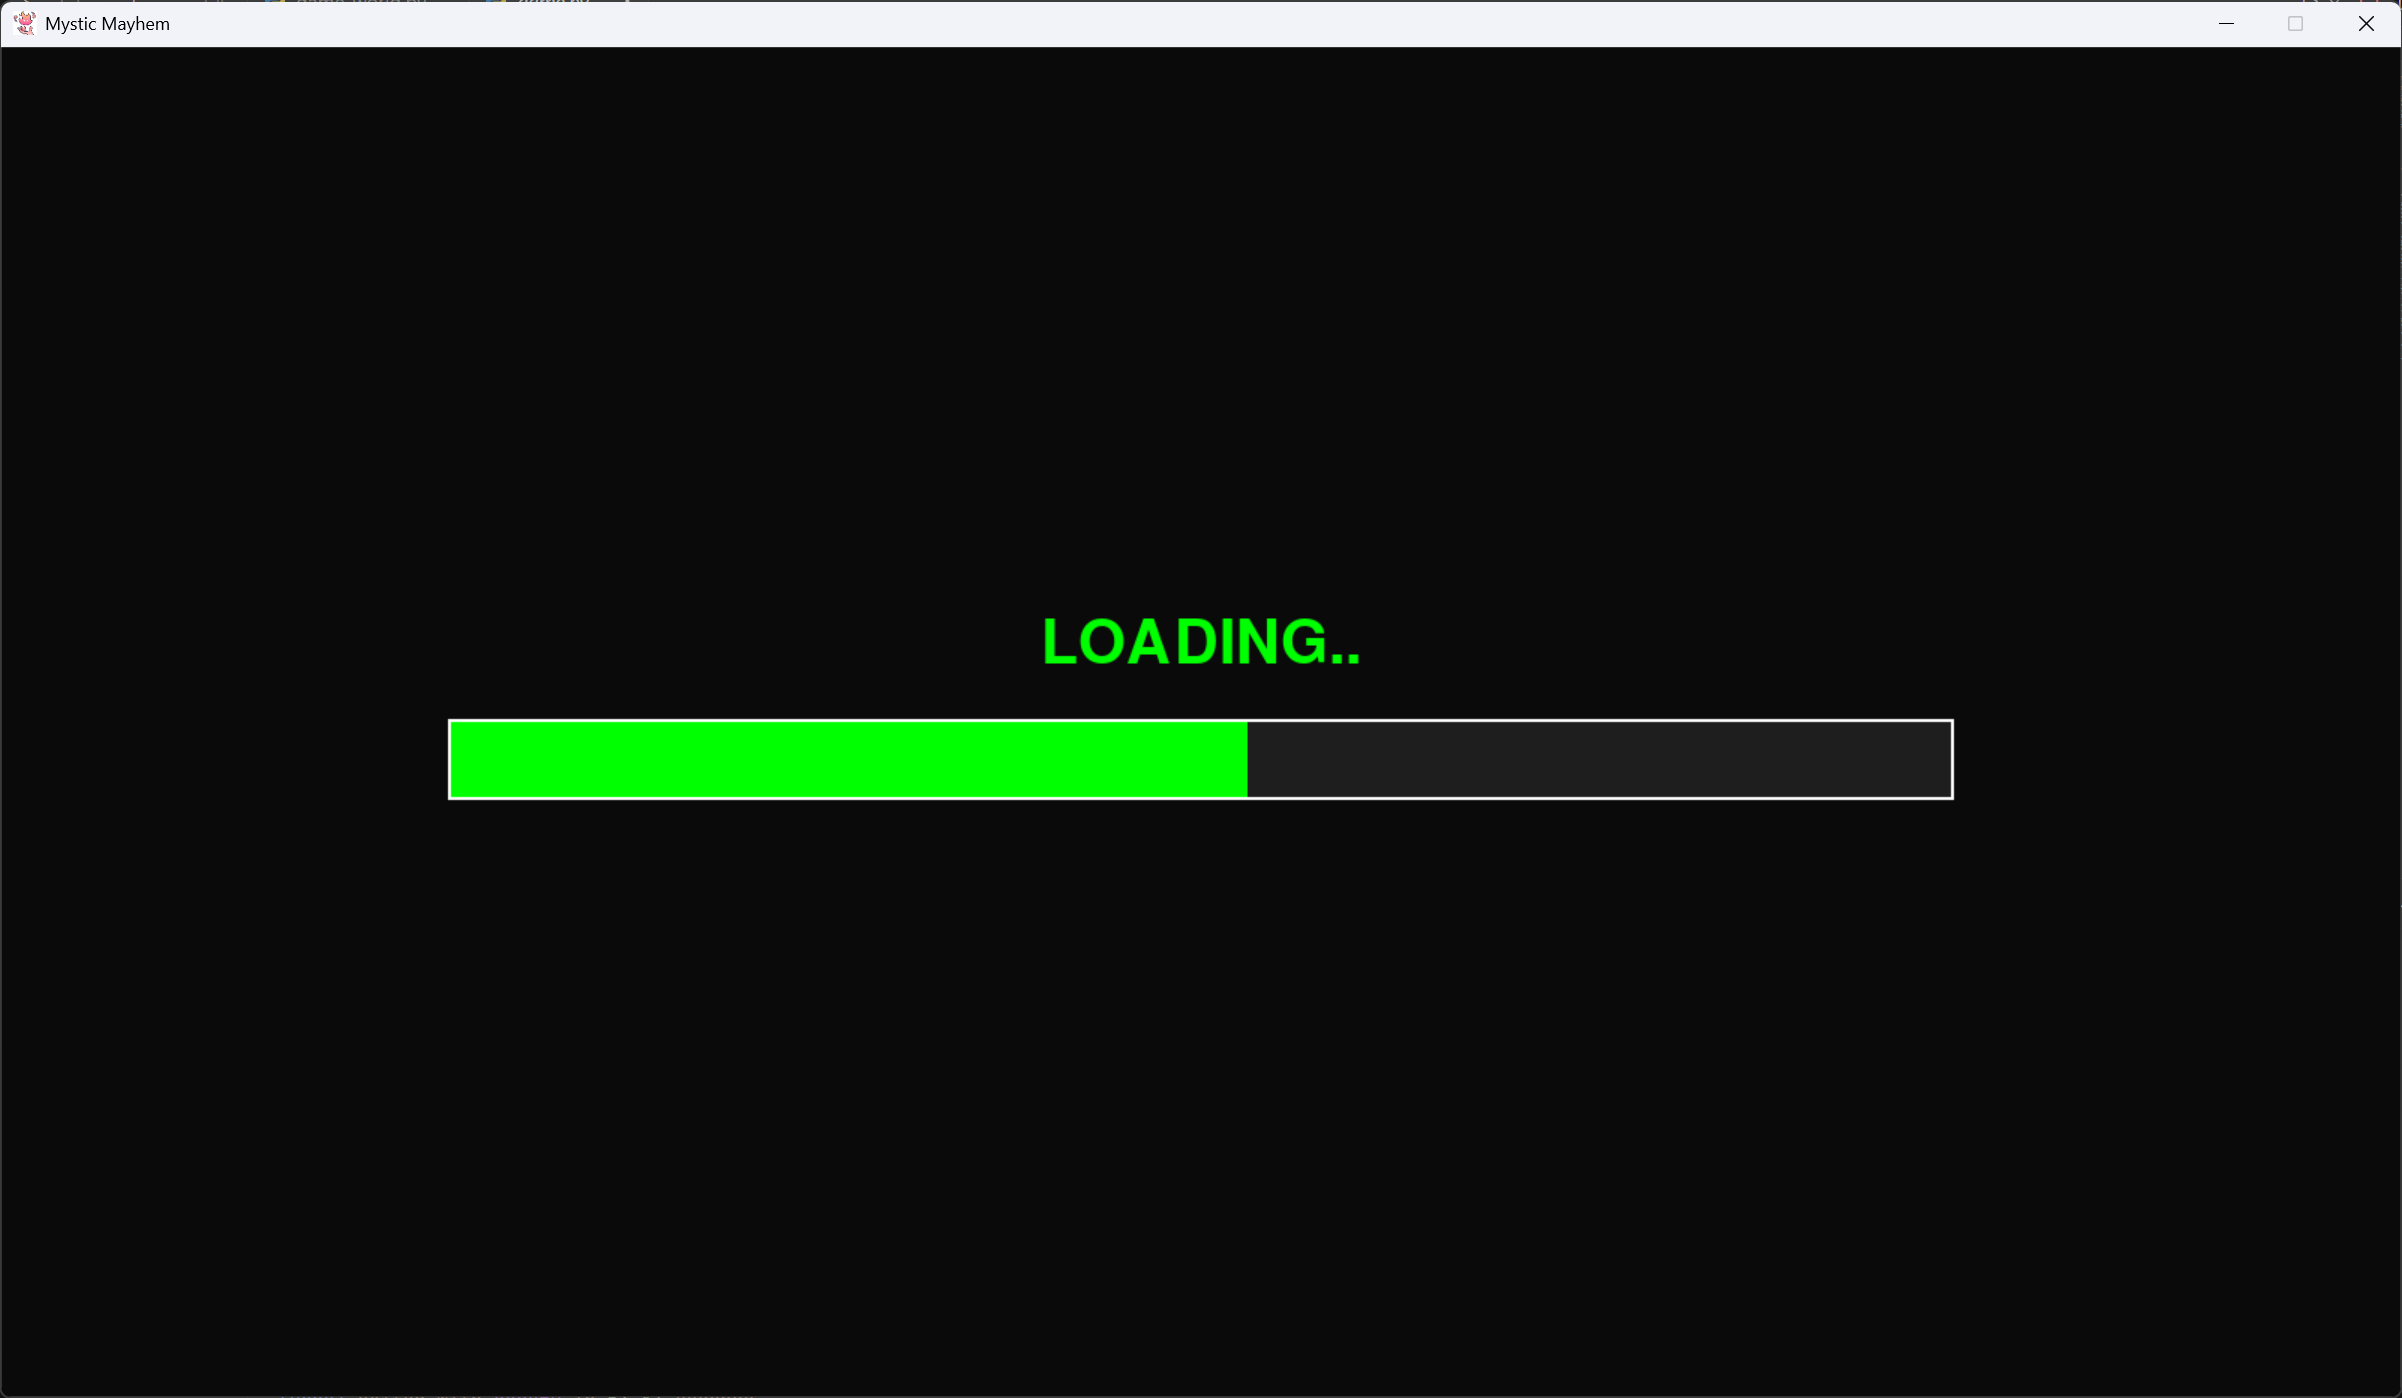
\includegraphics[width=\textwidth]{loading.png}
        \caption{Loading Screen}
        \label{fig:image1}
    \end{minipage}
    \hfill
    \begin{minipage}[t]{0.45\textwidth}
        \centering
        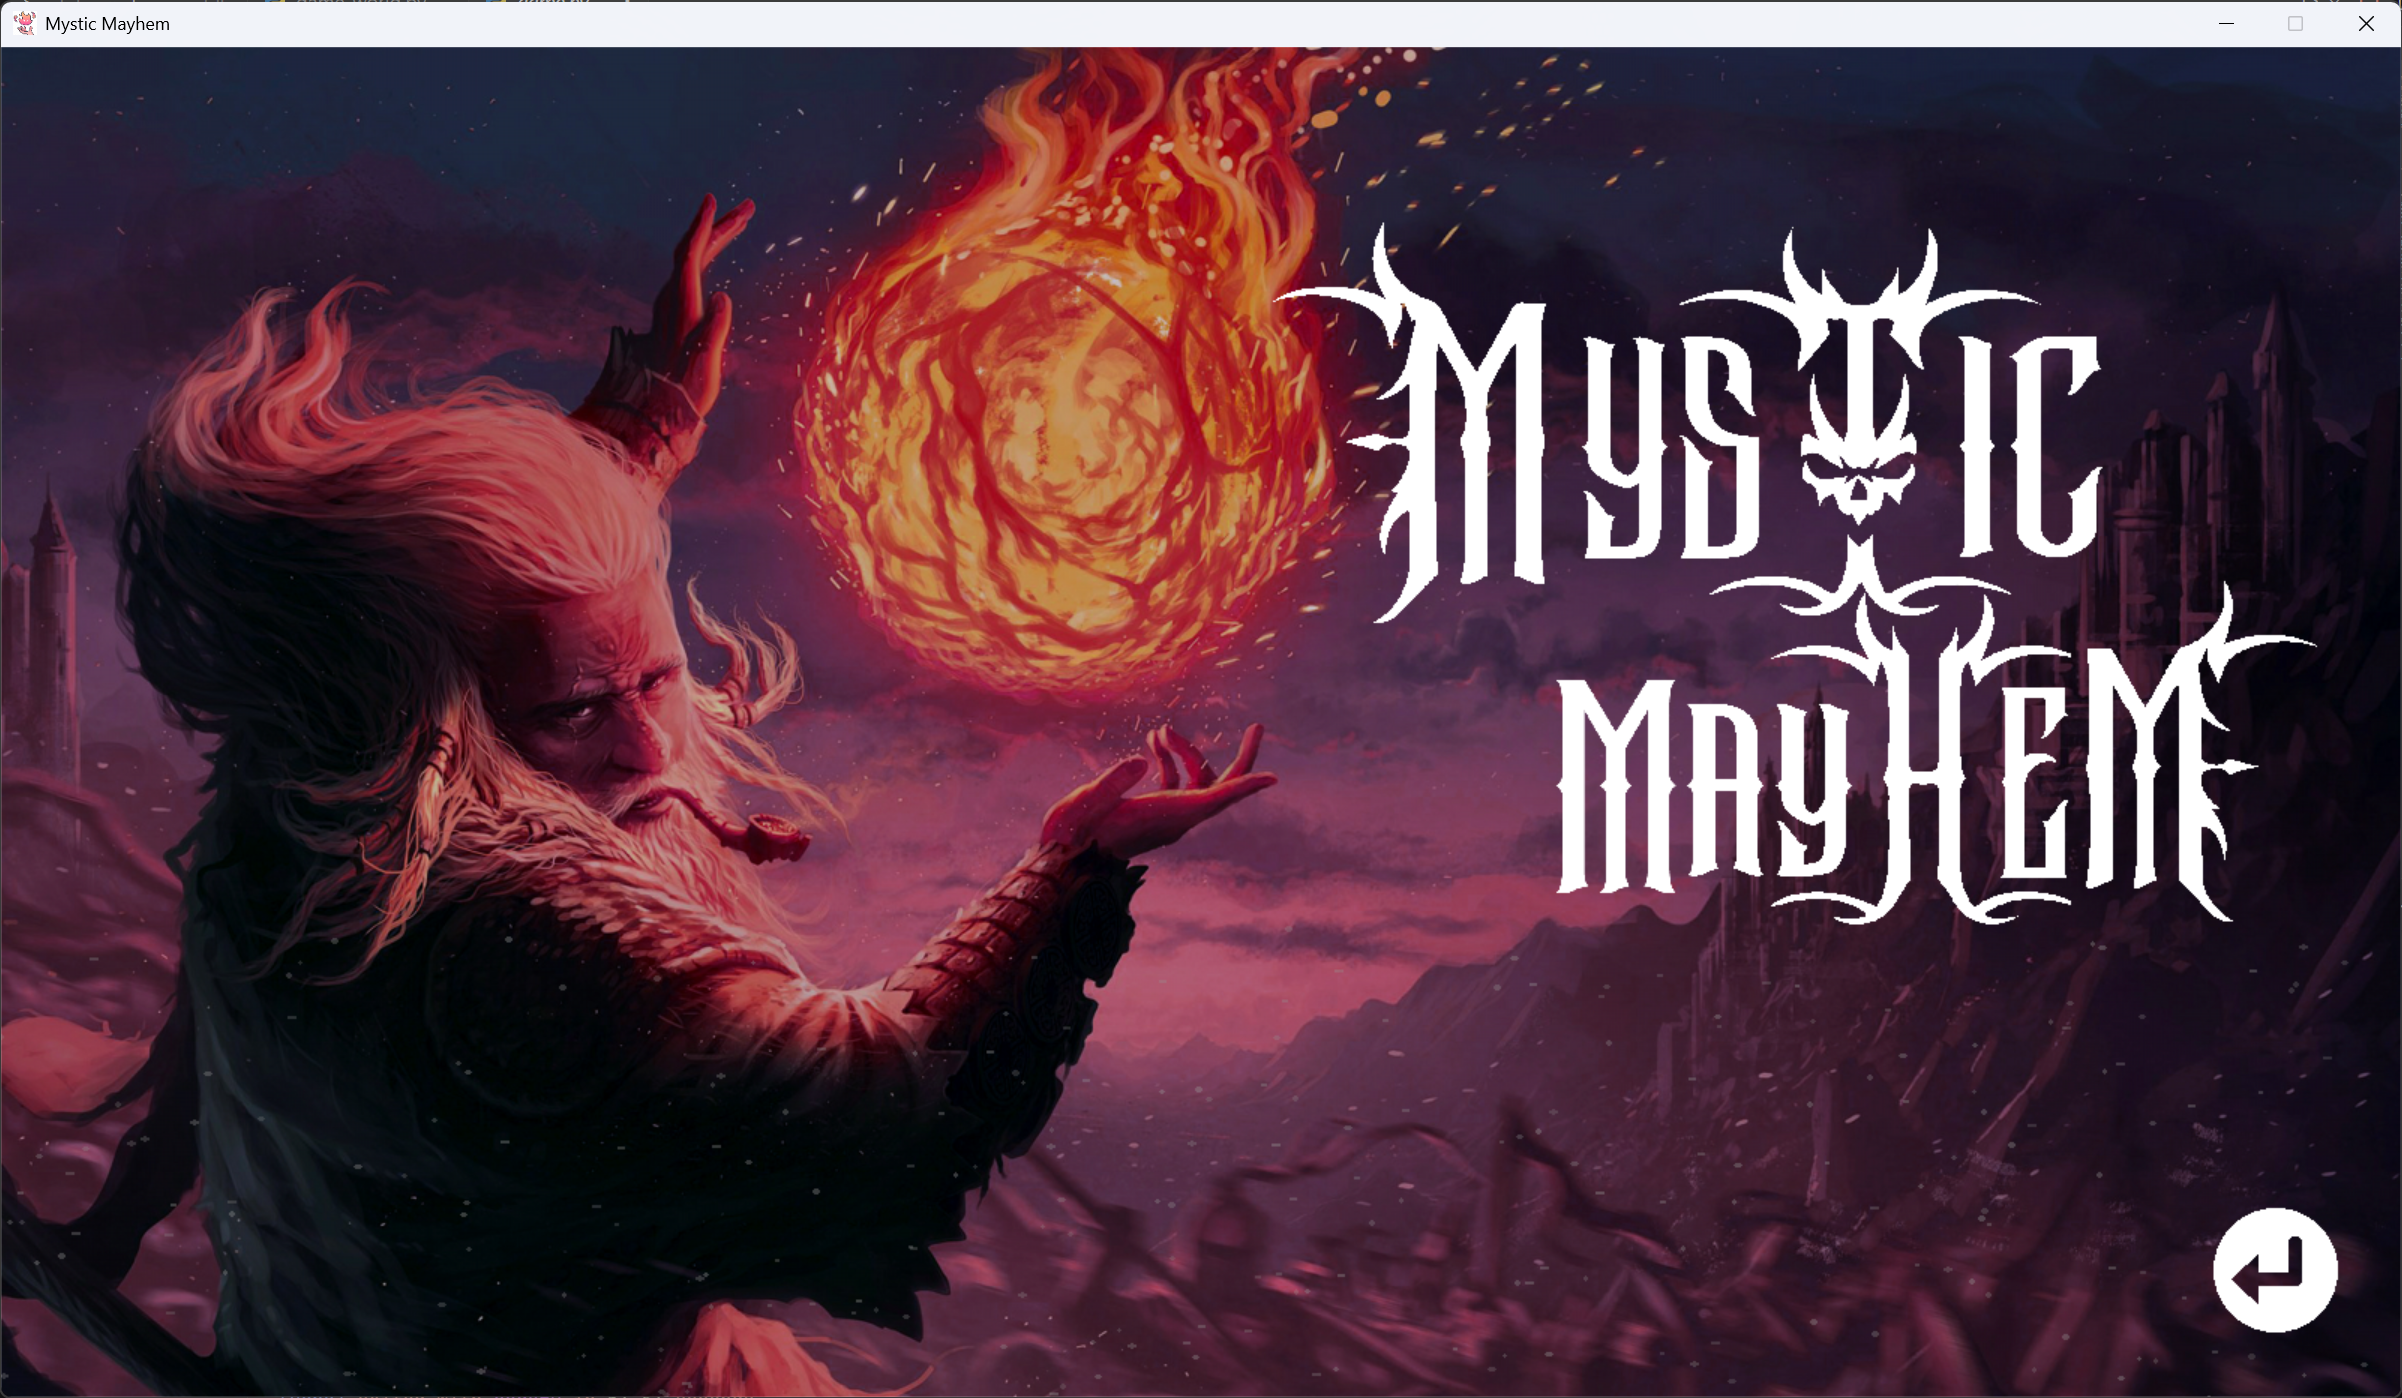
\includegraphics[width=\textwidth]{intro.png}
        \caption{Intro Screen}
        \label{fig:image2}
    \end{minipage}
\end{figure}

\subsubsection{Main Menu}
After Loading, you will be greeted with a Main Menu, from which you can choose to:
    \begin{itemize}
        \item Start Game
        \item Options to change Volume of music and sound effects, change resolution of the game window, or to view the tutorial
        \item Credits
        \item Leaderboard to view ranking of all players
    \end{itemize}
    You can select any of these by pressing on these buttons by mouse or using arrow keys and pressing Enter key to press. To exit, Press the Esc key or close the pygame window
    \vspace{0.2cm}
    \begin{figure}[h!]
        \centering
        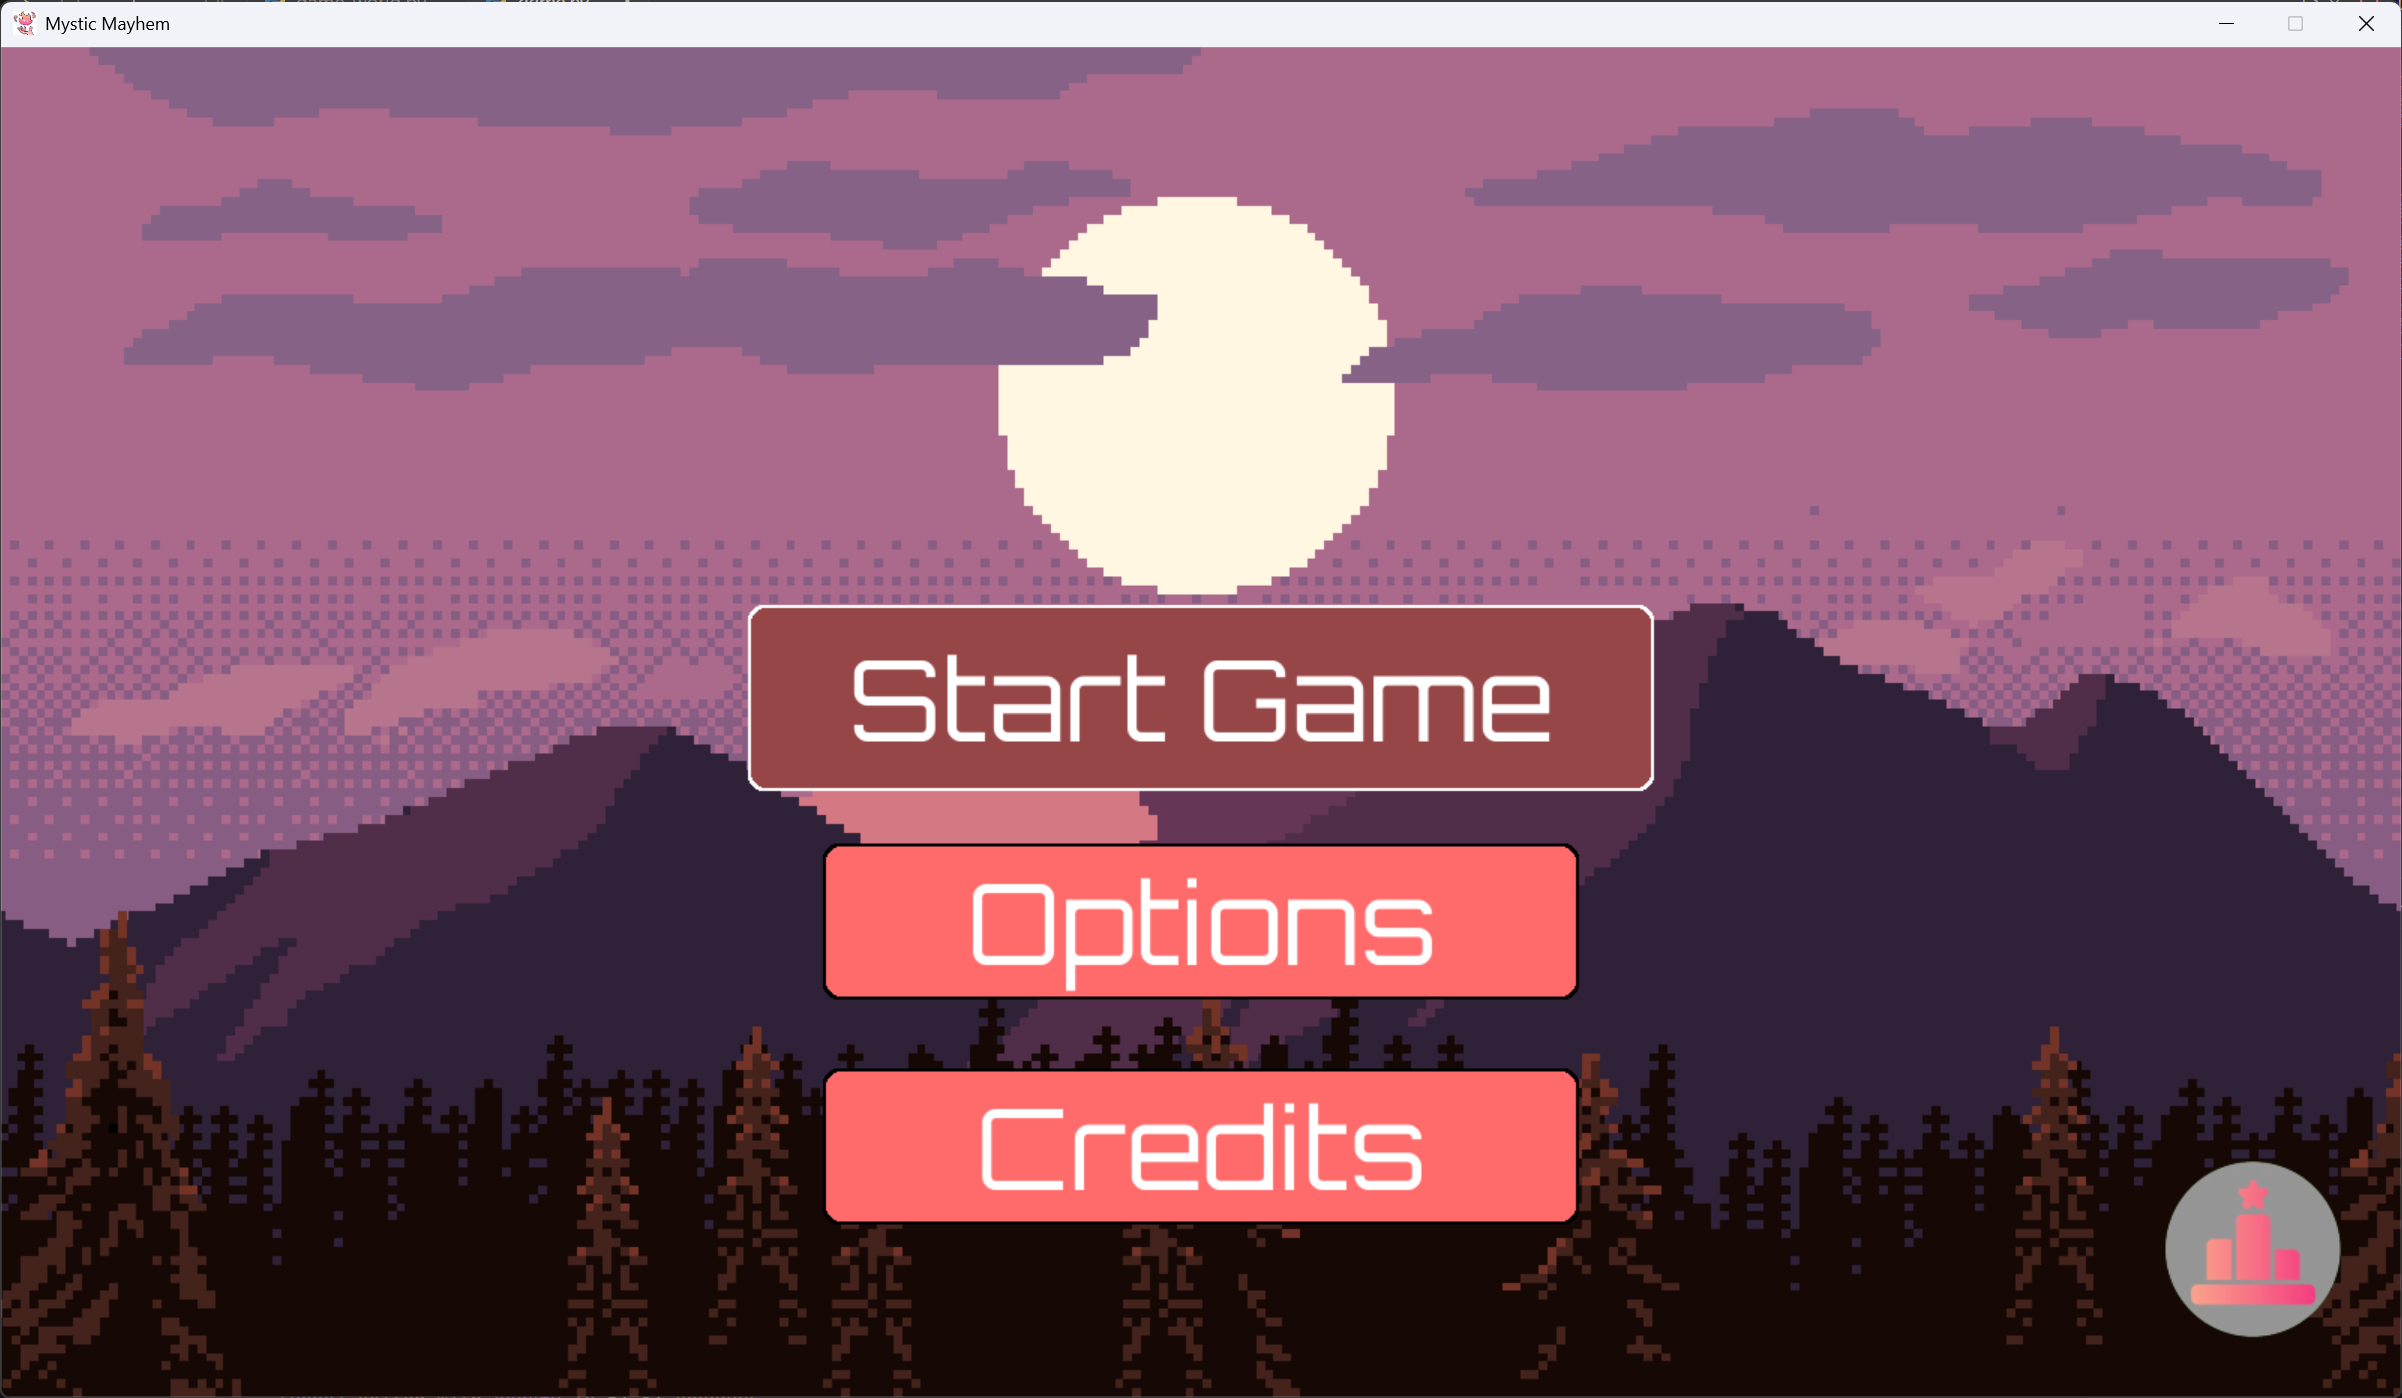
\includegraphics[width=0.8\textwidth]{mainmenu.png}
        \caption{Main Menu}
        \label{fig:MainMenu}
    \end{figure}

\newpage

\subsubsection{Tower Selection}
Clicking on Start Game will lead you to the name input and tower selection page where you will be required to type your name and select your desired tower structure, you can also select random tower in which the game would randomly choose a tower for you. One more thing to add is you can also leave the name empty, the game would select one of the default names in such a case.To confirm the selection press ready.
    \begin{figure}[h!]
        \centering
        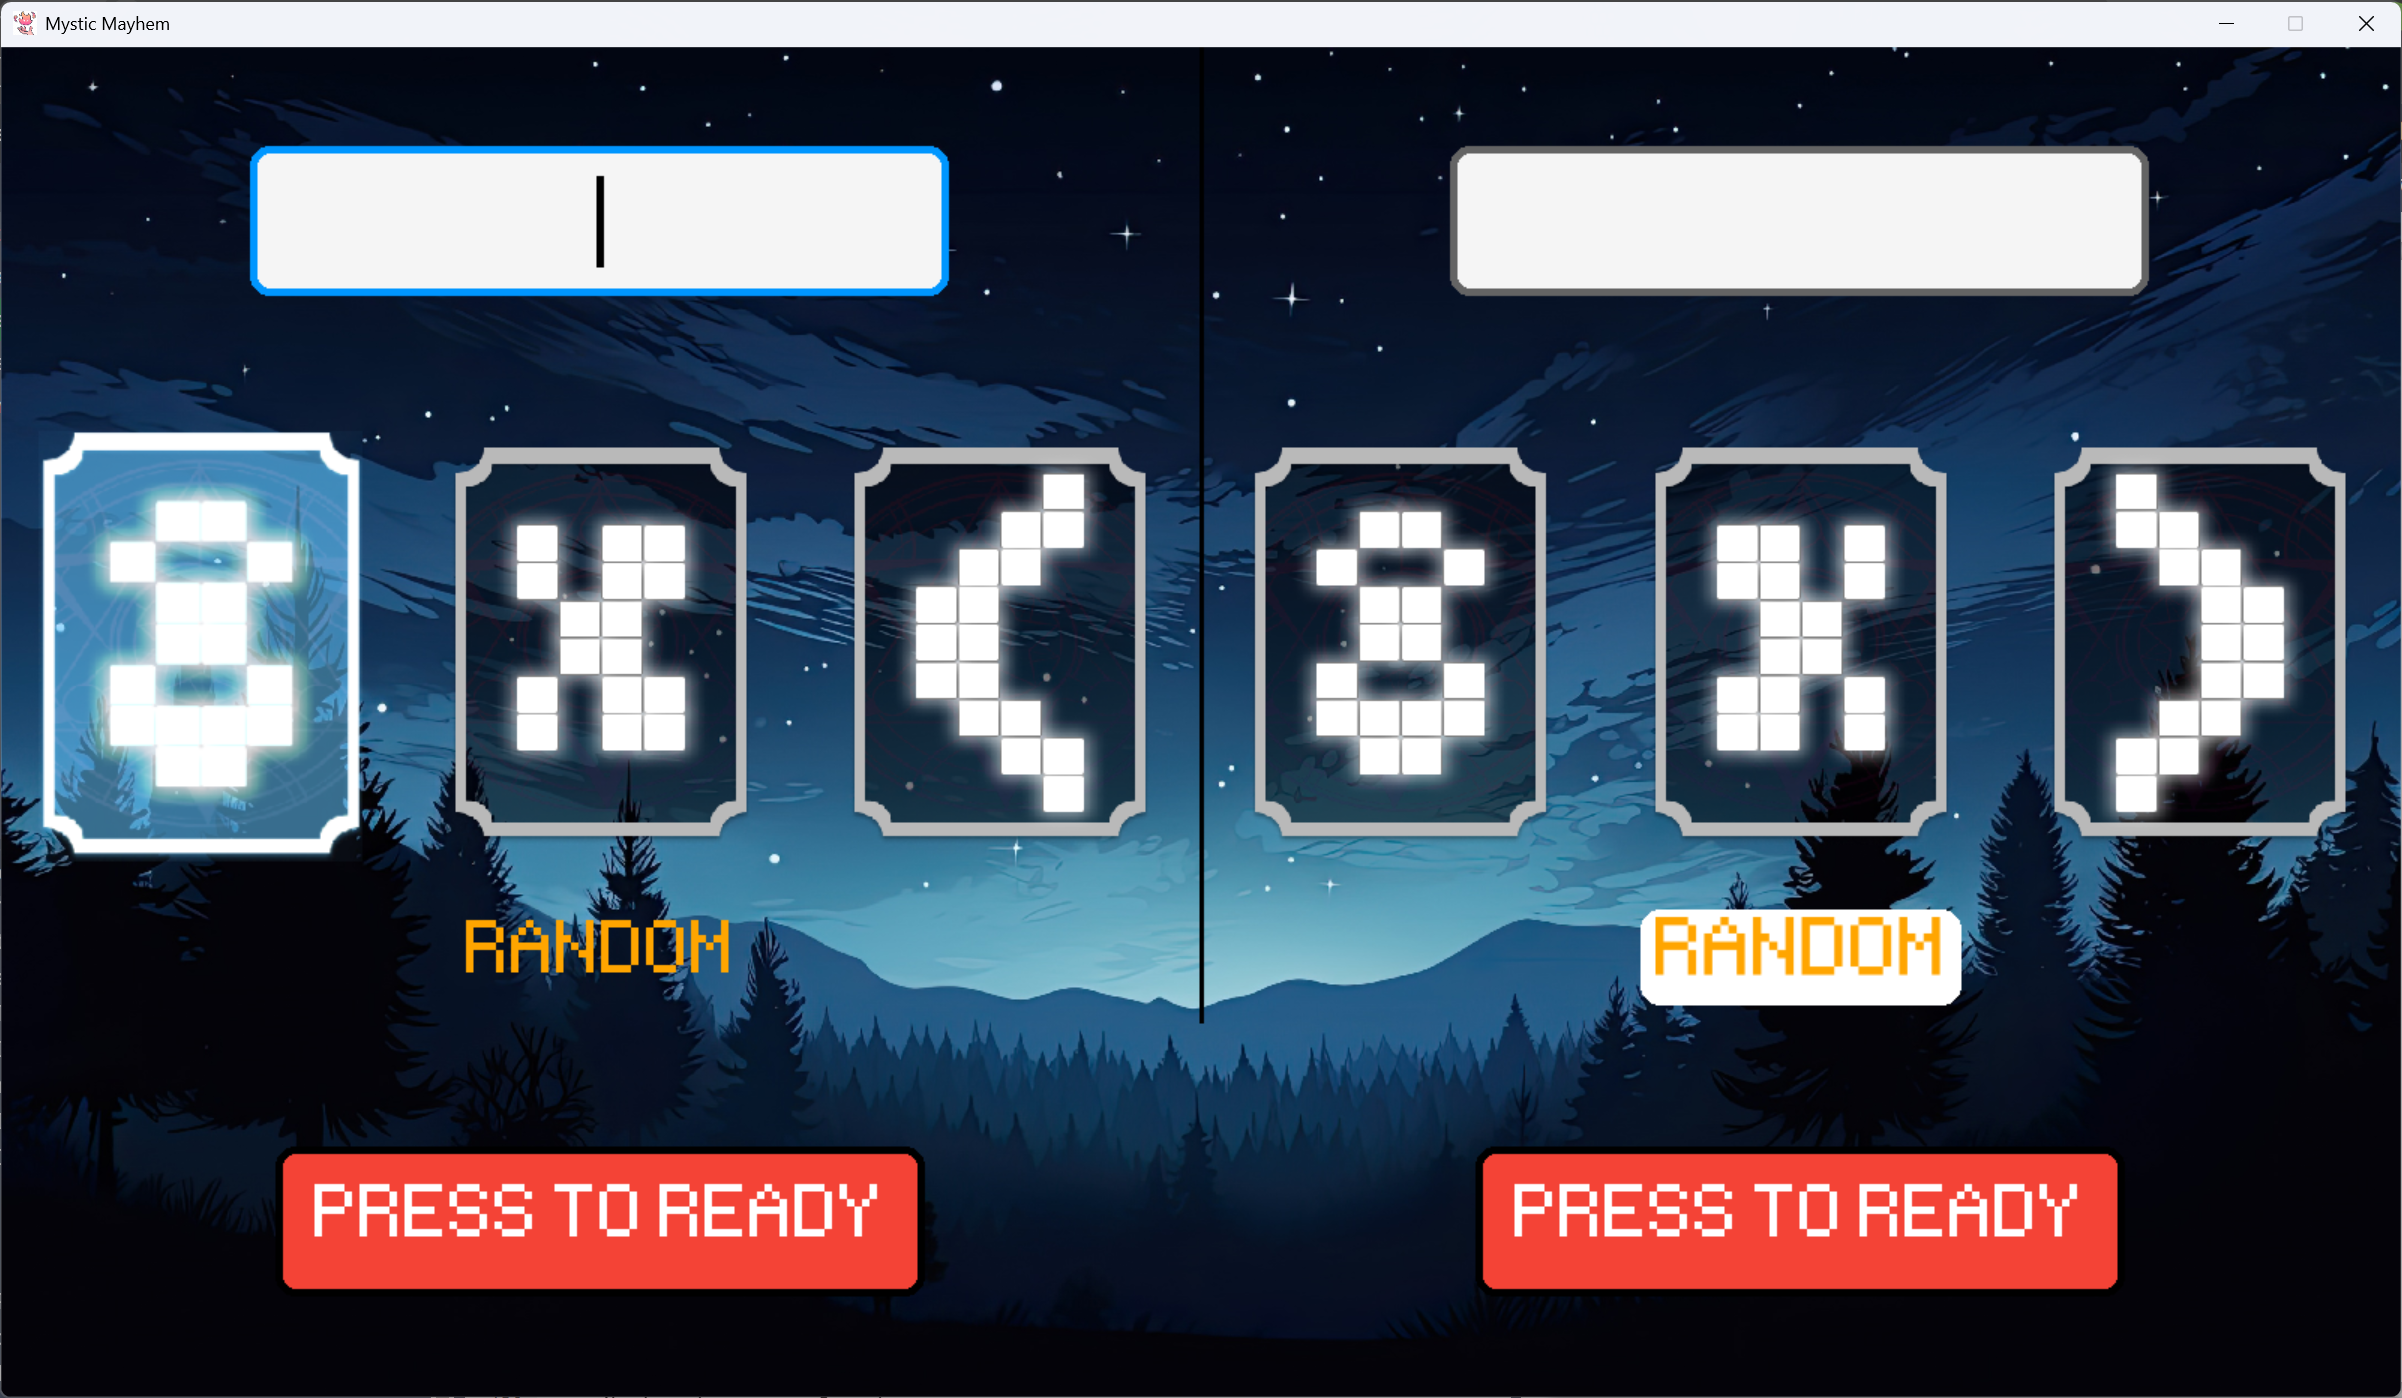
\includegraphics[width=0.5\textwidth]{select.png}
        \caption{Select Screen}\label{fig:select}
    \end{figure}

\subsubsection{Game World}
Once both players are ready, the game starts after a 3 second countdown, leading to the main game world, a 1v1, turn based battle inspired by Angry Birds, set in a wizard themed fantasy world. Players take turns selecting a spell and launching a magical orb at the opponent's tower by dragging in the desired direction. Upon release, the orb is affected by gravity and air drag. If you begin dragging but decide not to throw, you can reposition the orb to the center and release the mouse to cancel the action. \\
When the orb hits a block in the opponent's tower, it deals damage to that block and the adjacent blocks in the four cardinal directions. You can also trigger the orb's explosion manually in mid air by right clicking or pressing the “O” key, causing area damage to nearby blocks. \\
The goal is to strategically demolish all the blocks in the opponent's tower to win the match.

\begin{figure}[h!]
    \centering
    \begin{subfigure}[b]{0.35\textwidth}
        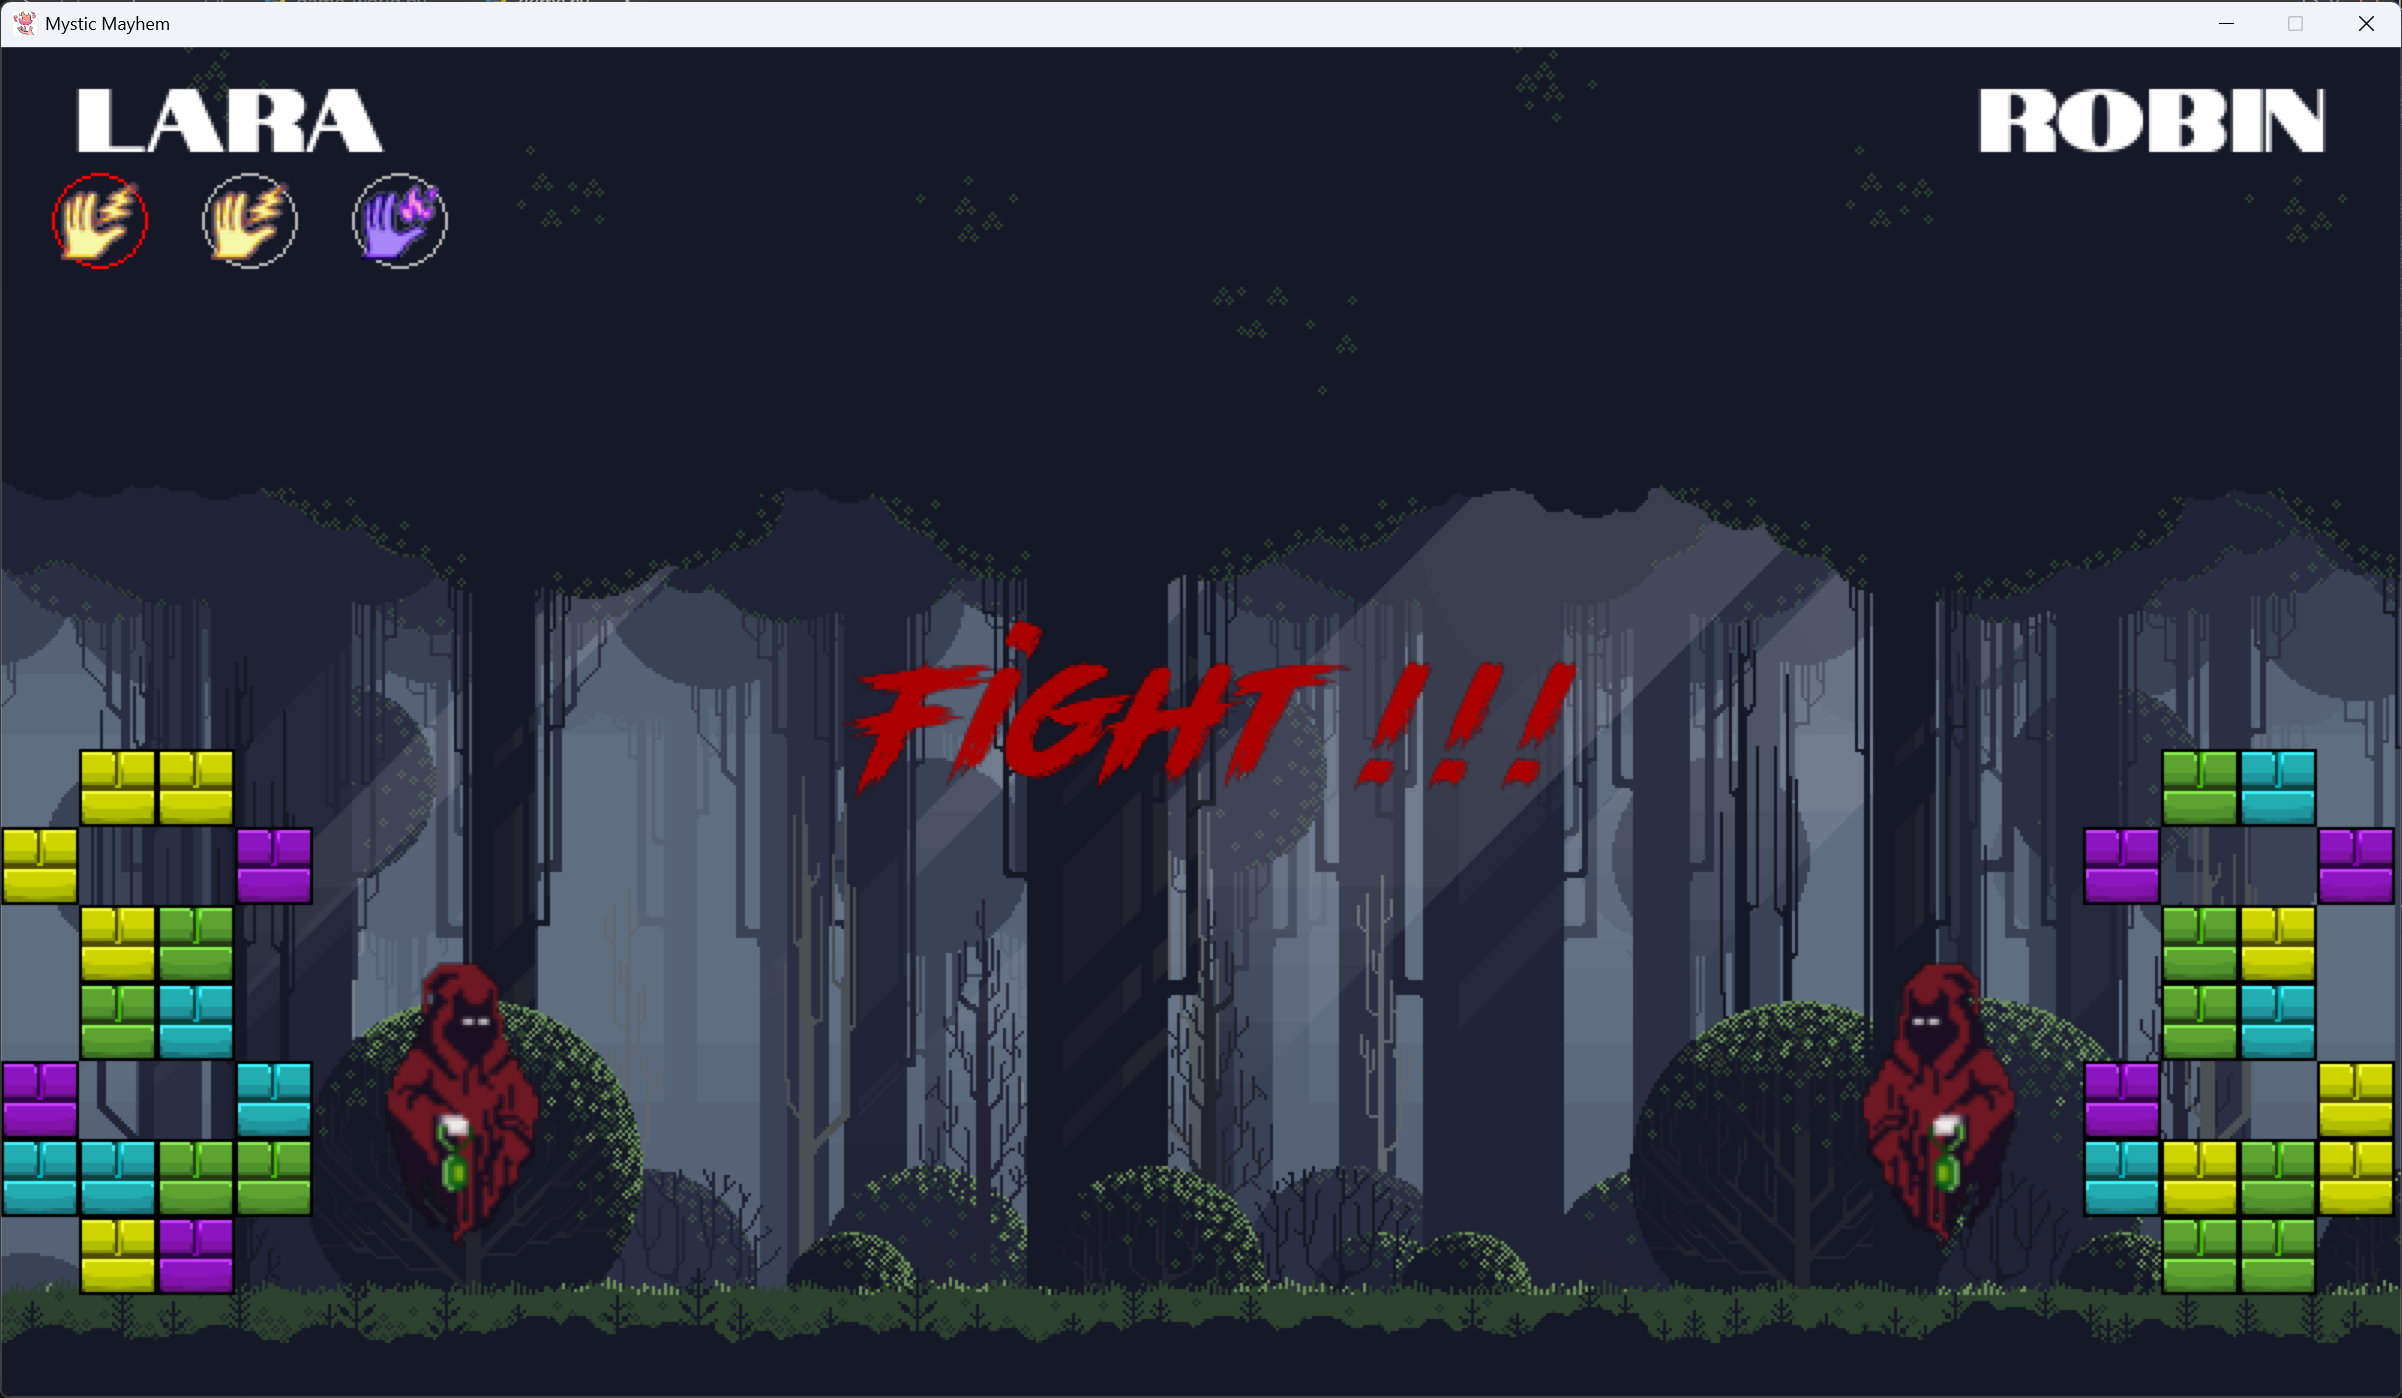
\includegraphics[width=\textwidth]{game1.png}
        \caption{Start}
        \label{fig:image1}
    \end{subfigure}
    \hfill
    \begin{subfigure}[b]{0.35\textwidth}
        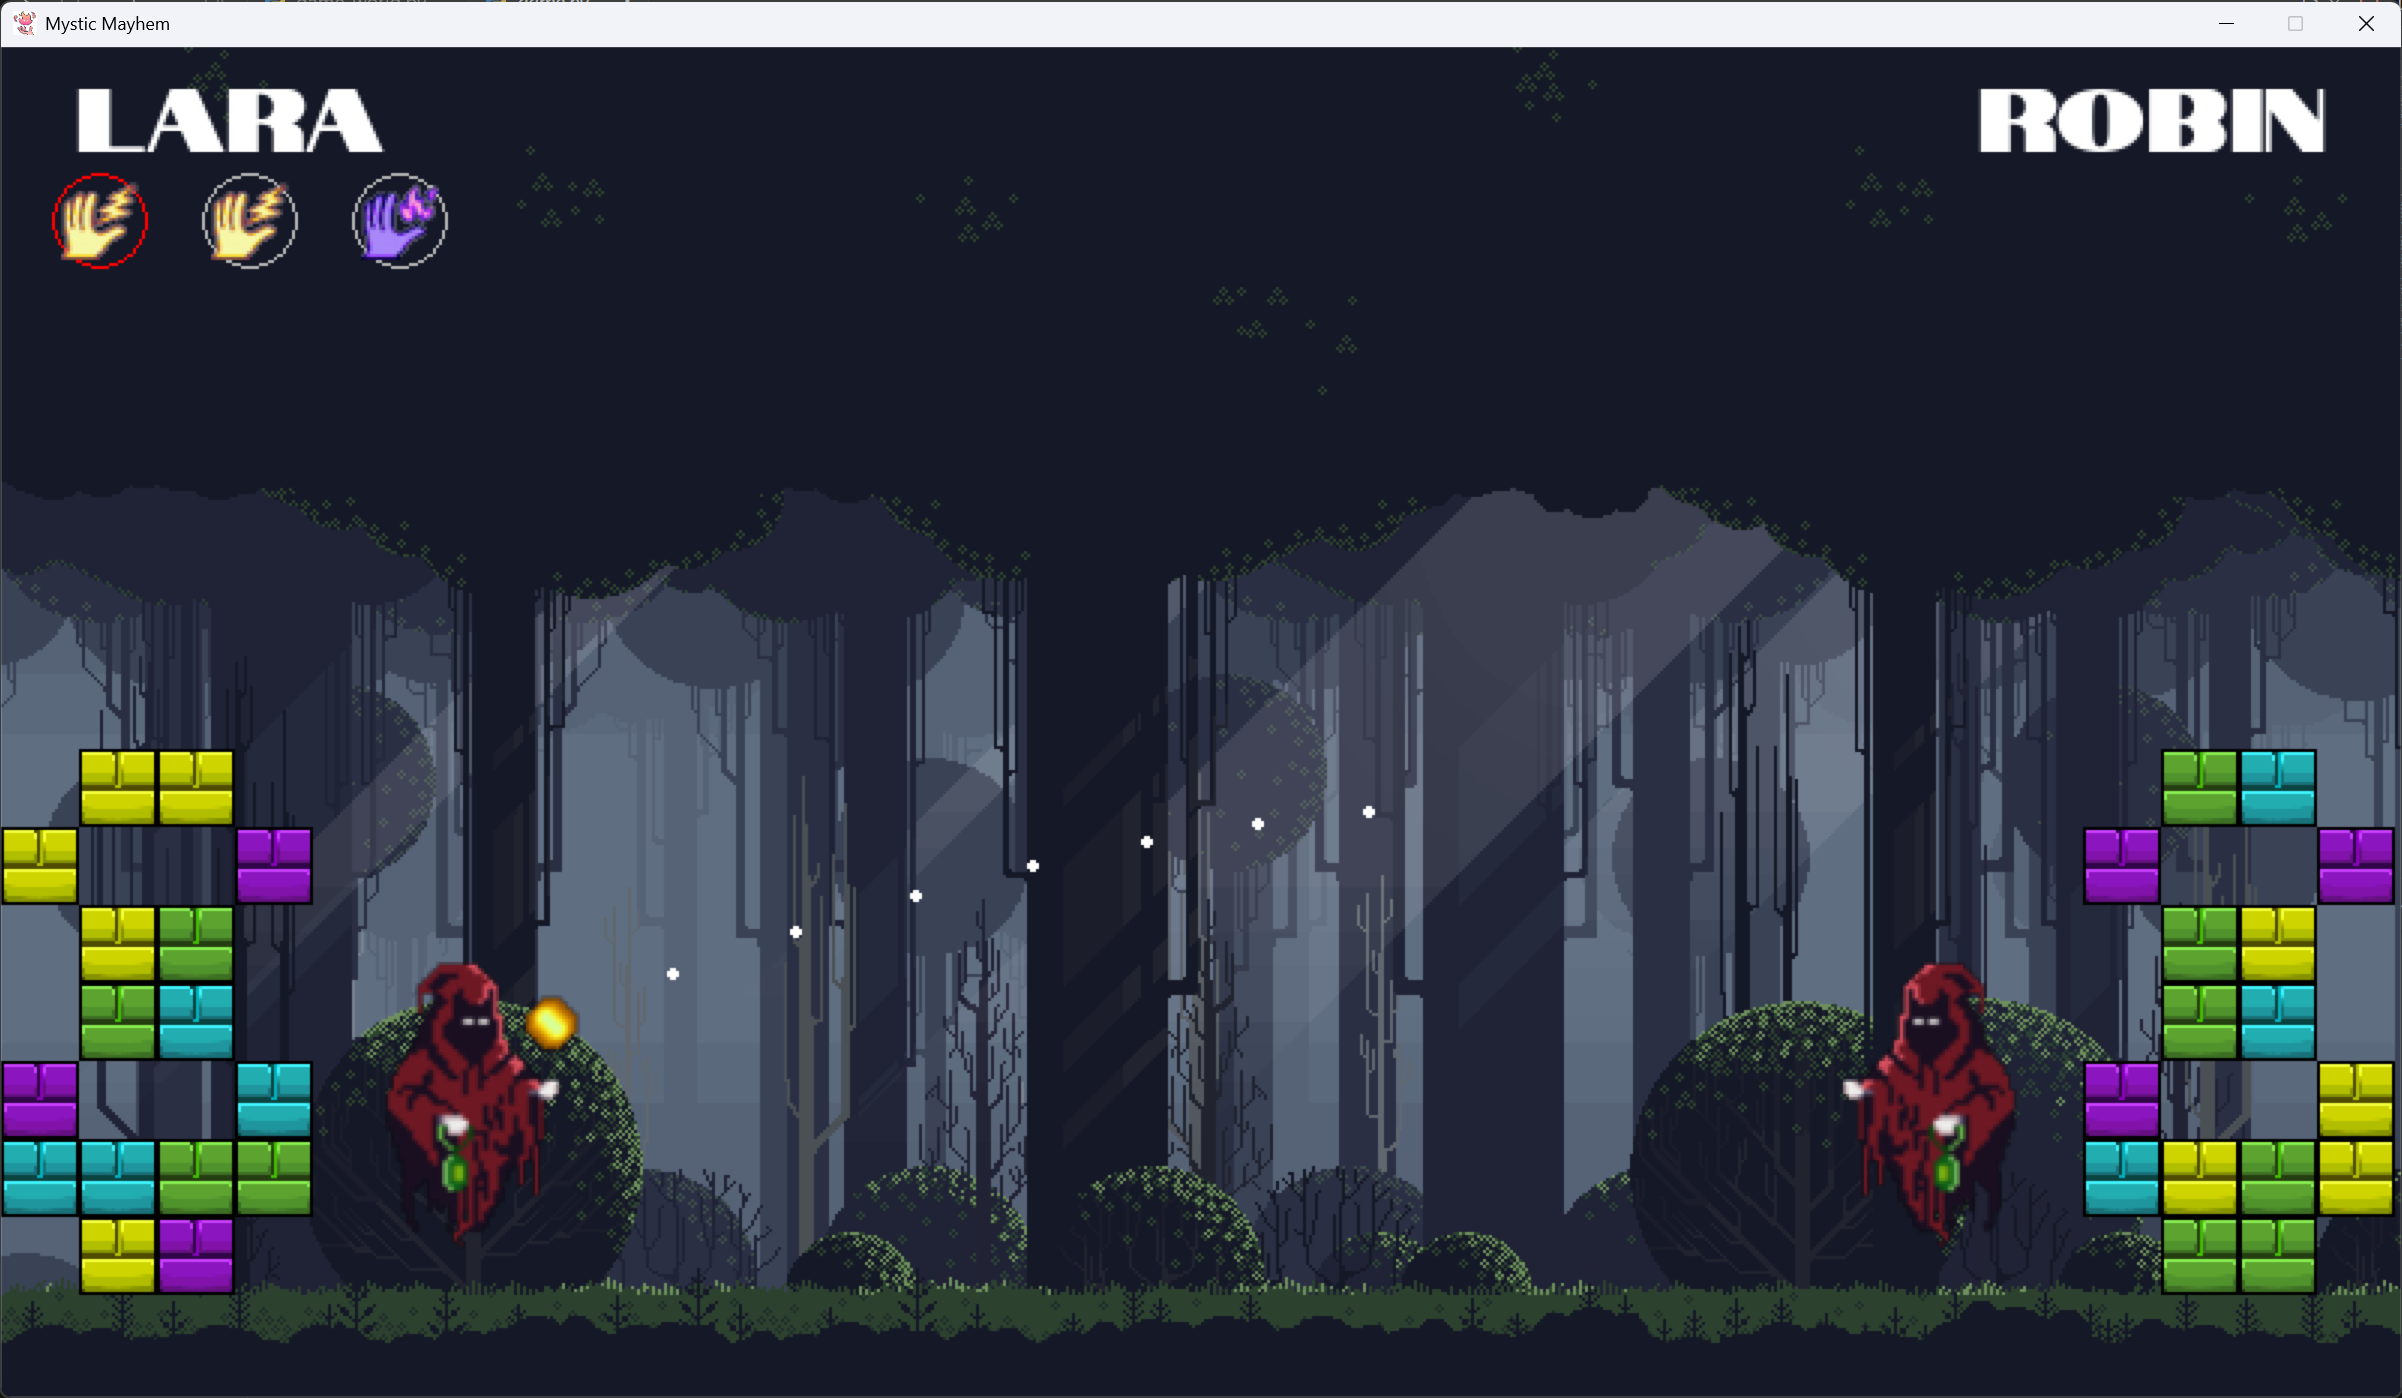
\includegraphics[width=\textwidth]{game2.png}
        \caption{Launch}
        \label{fig:image2}
    \end{subfigure}
    \vskip\baselineskip
    \begin{subfigure}[b]{0.35\textwidth}
        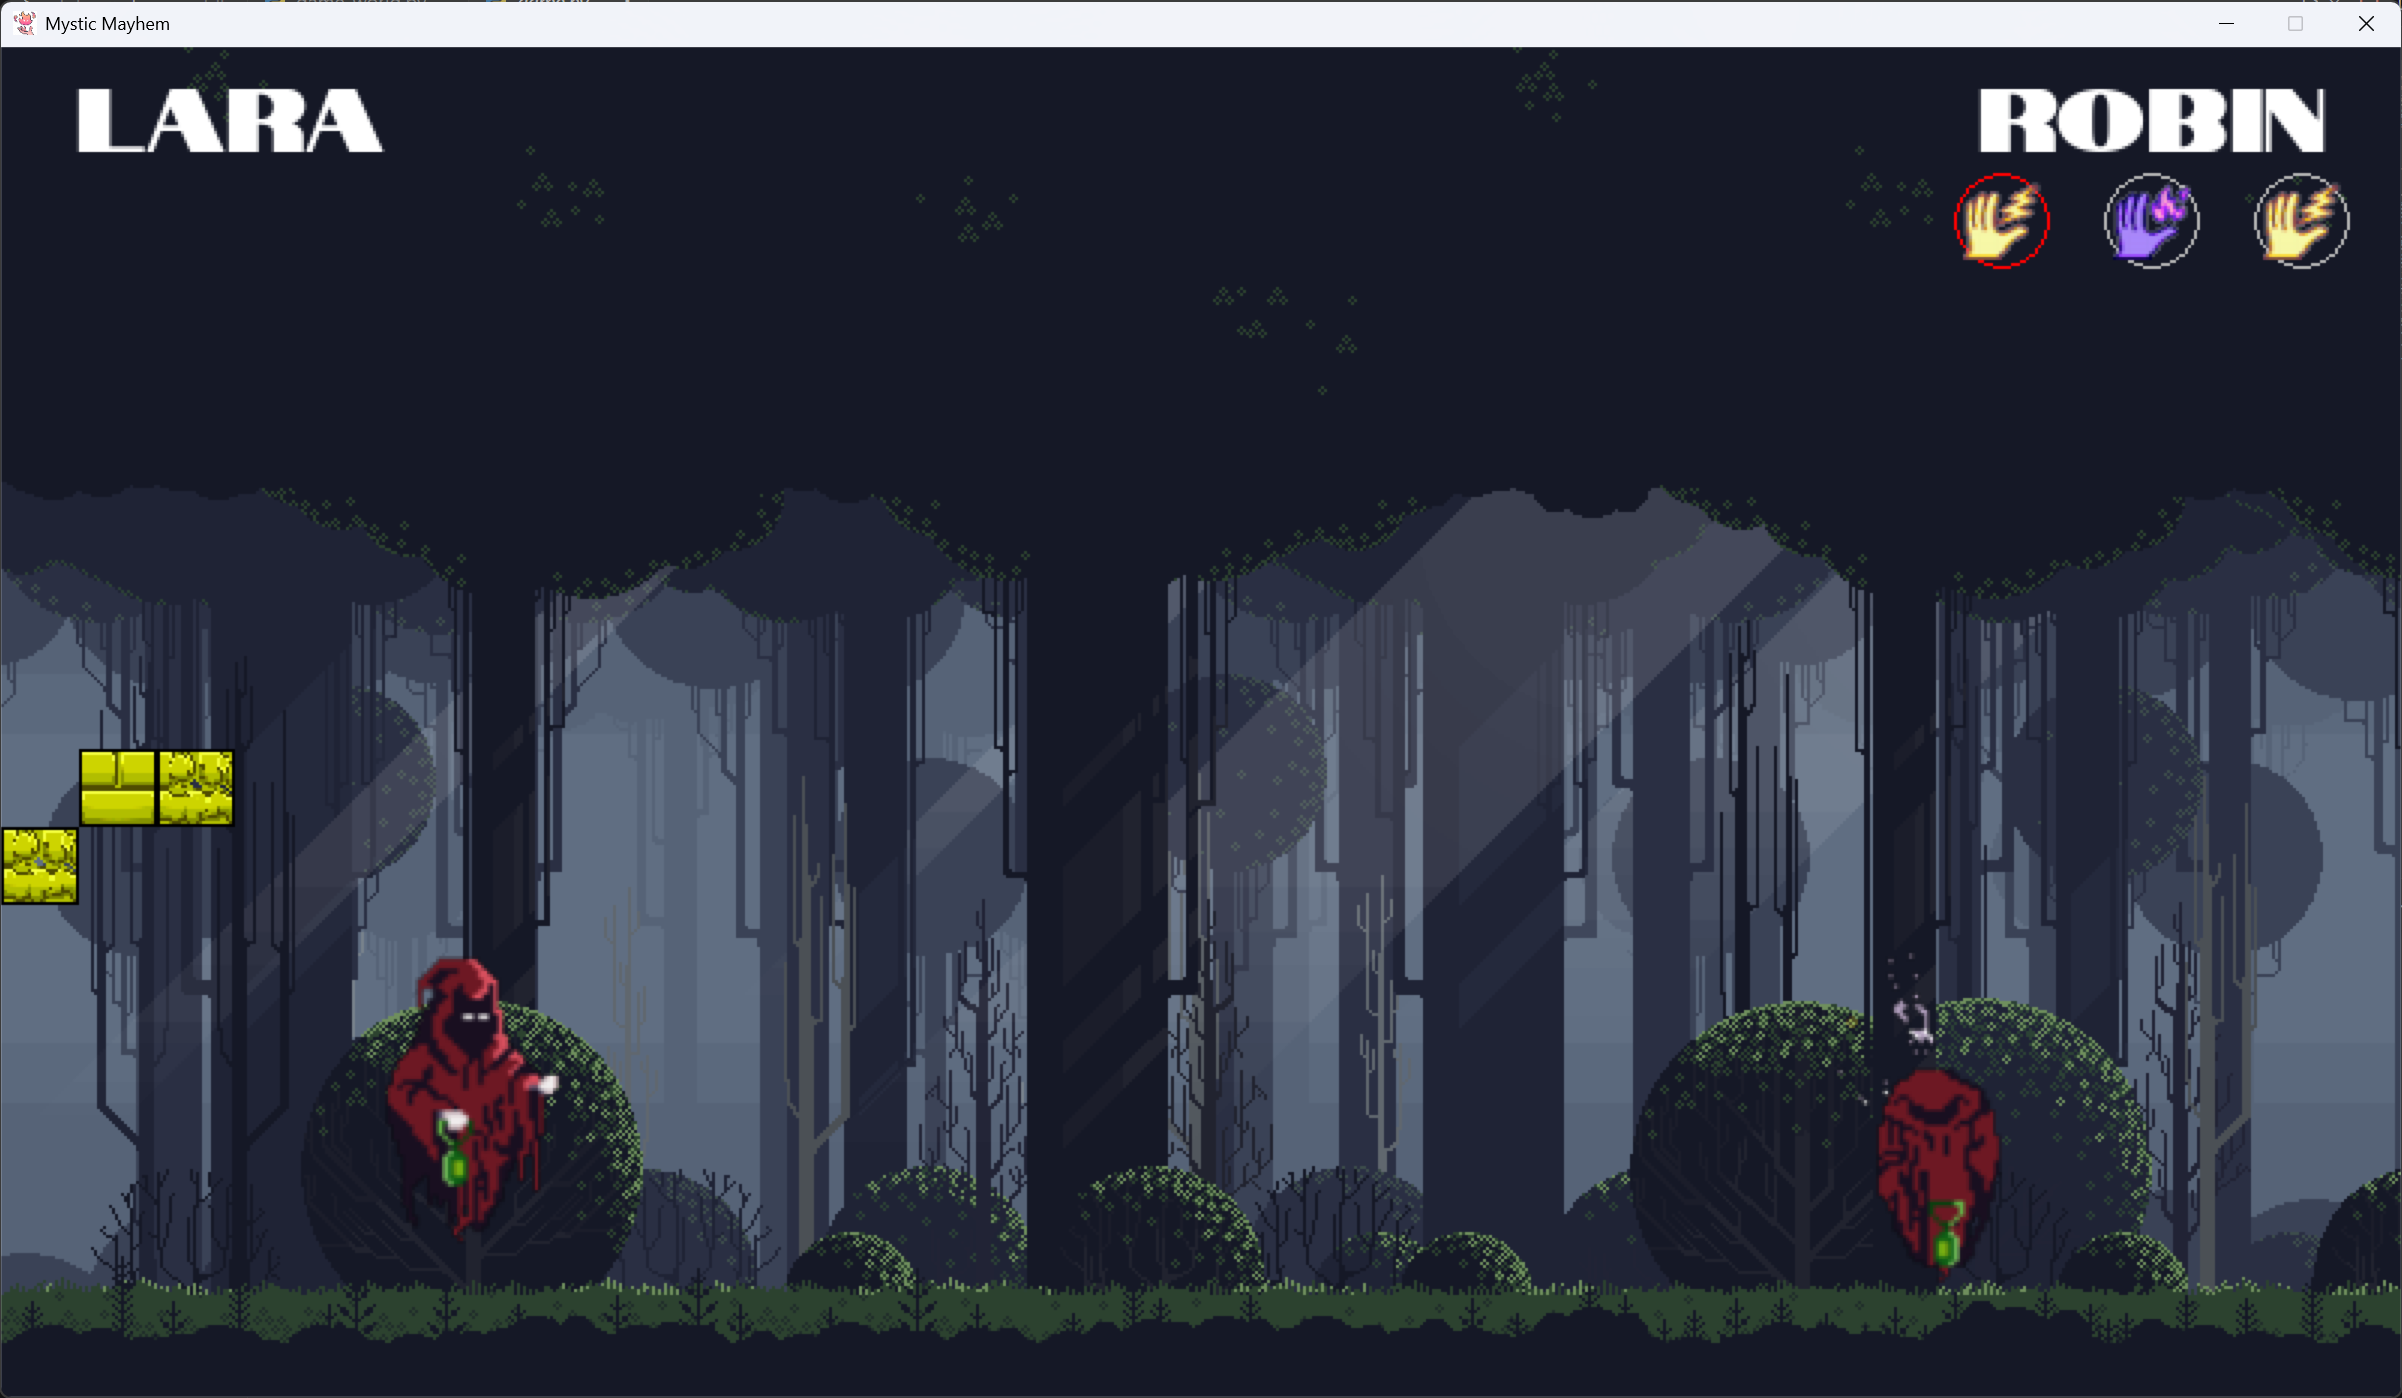
\includegraphics[width=\textwidth]{game3.png}
        \caption{Death}
        \label{fig:image3}
    \end{subfigure}
    \hfill
    \begin{subfigure}[b]{0.35\textwidth}
        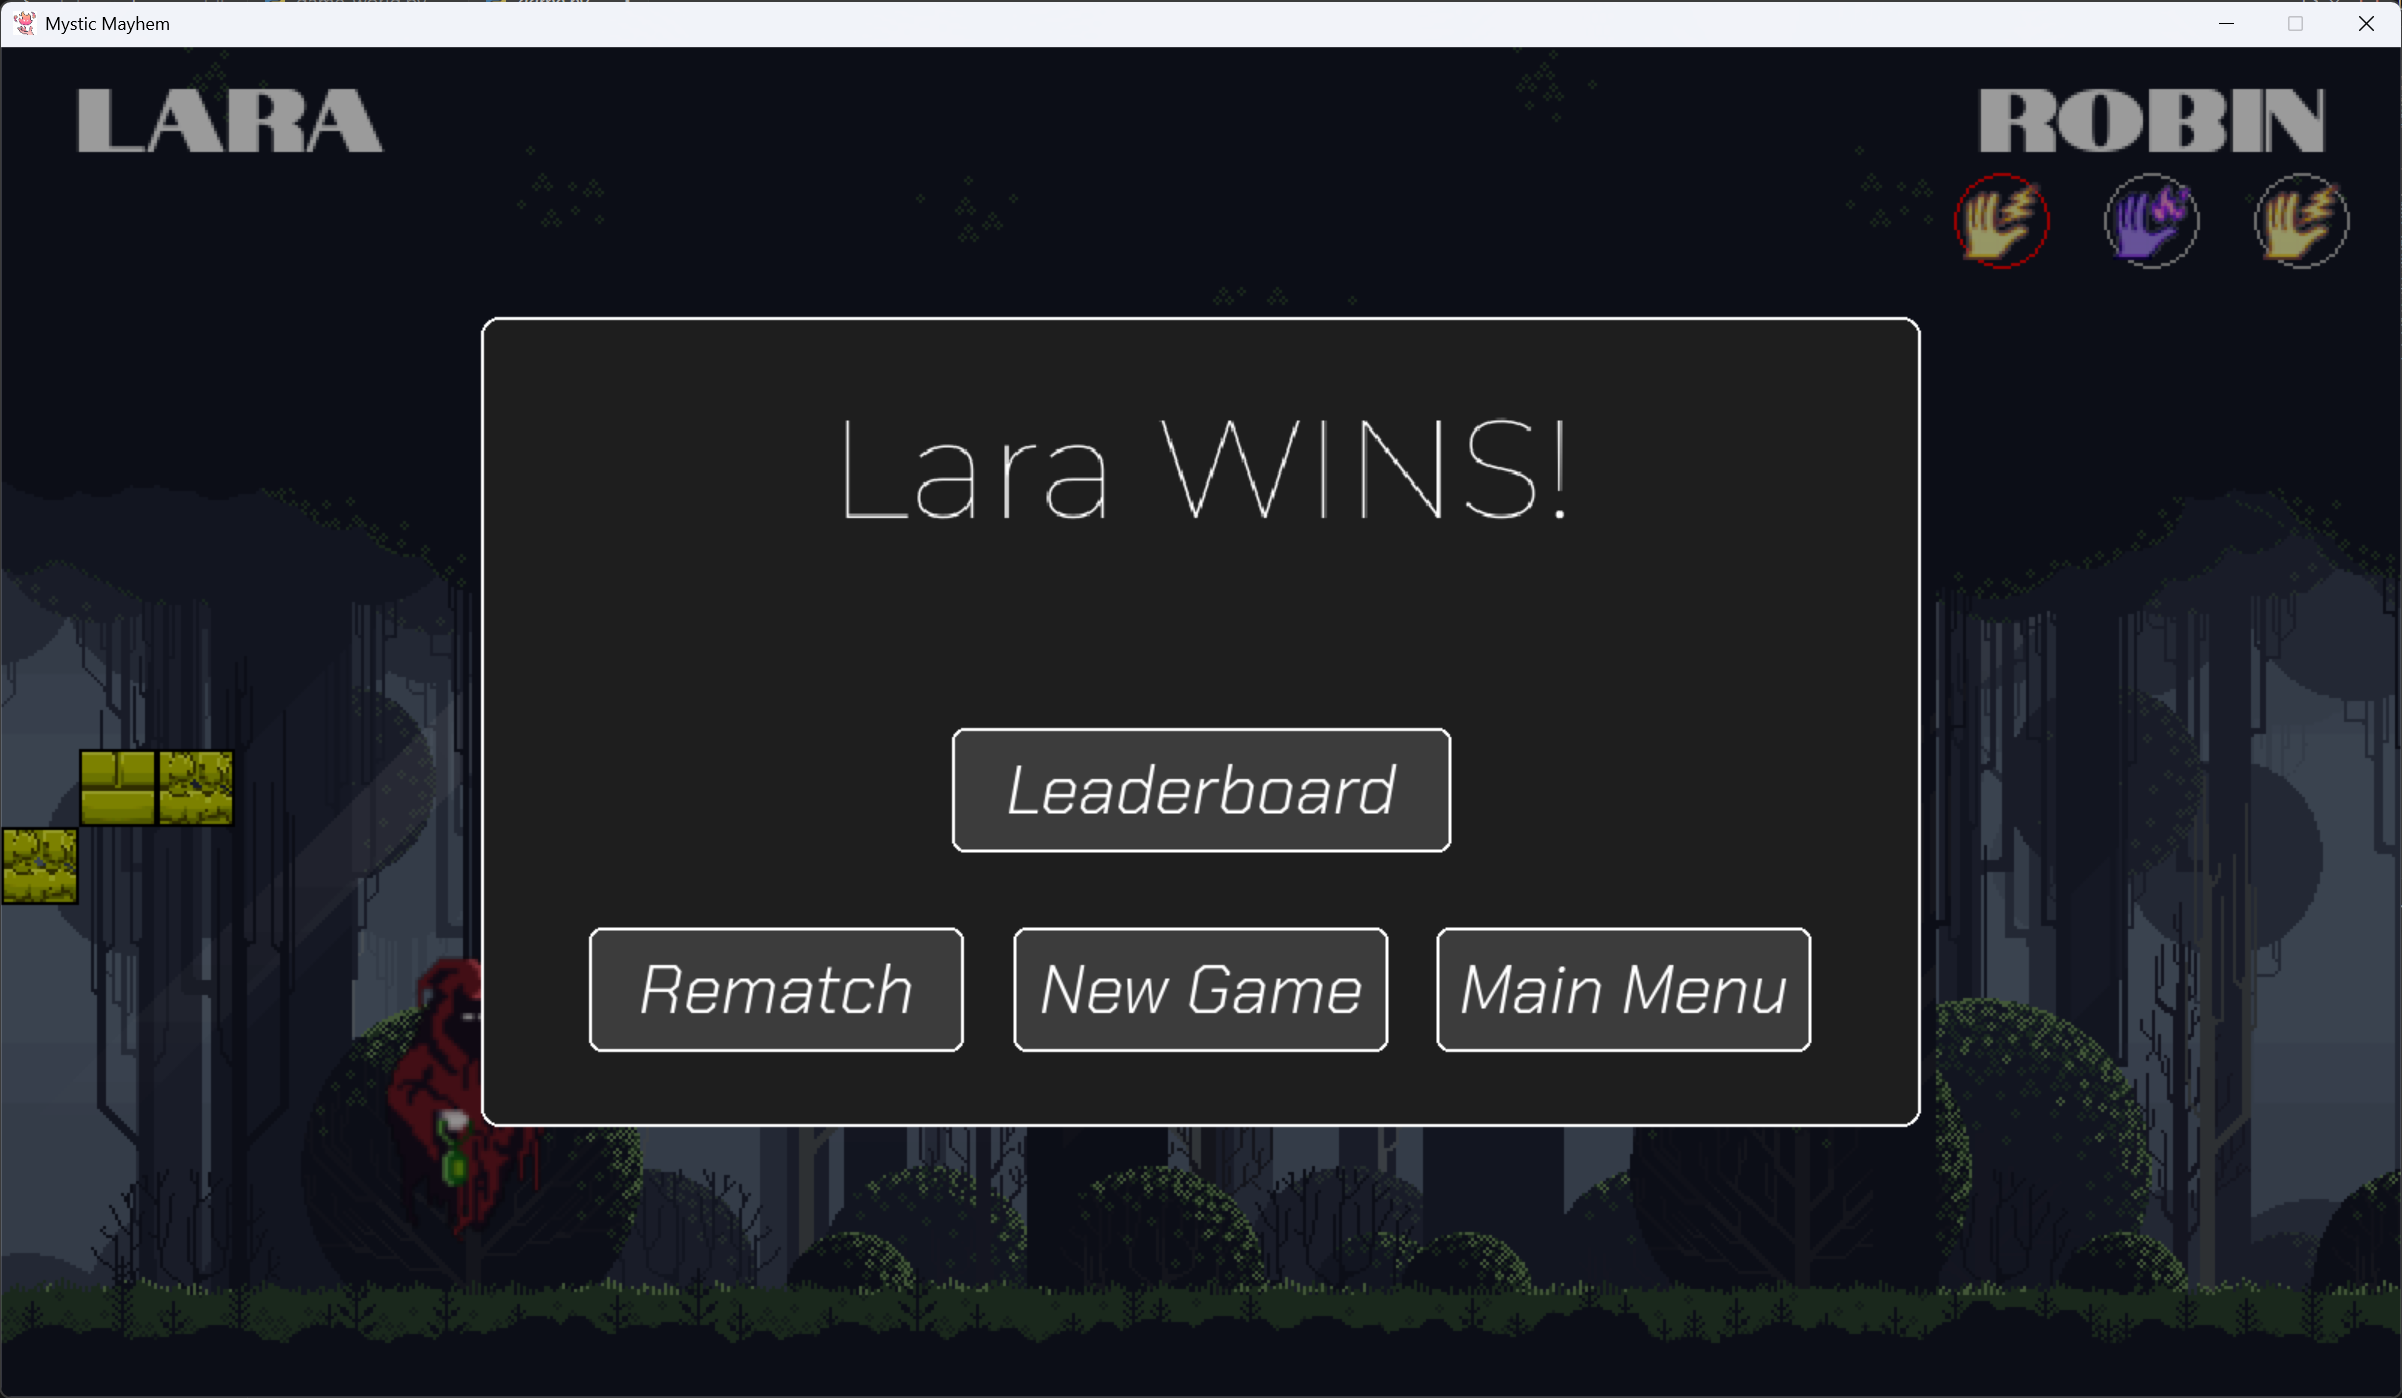
\includegraphics[width=\textwidth]{game4.png}
        \caption{End Screen}
        \label{fig:image4}
    \end{subfigure}
    \caption{Screenshots from different stages of the game world}
    \label{fig:2x2grid}
\end{figure}

\newpage

\subsubsection{Other Screens}
The game includes several additional screens and features that enhance the overall experience:
\begin{itemize}
    \item A pause menu can be accessed by pressing the \texttt{Esc} key, offering options to resume the game, return to the main menu, or adjust settings.
    \item The leaderboard displays detailed player statistics, including rankings, win/loss records, and the most frequently selected and best performing tower for each player.
    \item Various sound effects and smooth animations are integrated throughout the game to create an engaging and visually appealing experience.
    \item A tutorial section is available in the options menu, providing clear explanations of game mechanics and instructions on how to play.
\end{itemize}

\vspace{0.2cm}
\section{Key Implementation Details}

\subsection{Asset Loading}
All the assets including images with their desired dimensions, fonts with their desired size, and music are loaded all at once when the game start by defining list of assets to add and running it. For example:
\begin{lstlisting}[language=Python, caption={Image Loading}]
for img_file, alias, dim in self.image_files:
    path = os.path.join(self.sprite_directory, img_file)
    self.assets[alias] = LoadScaledImage(path, scaling_dim=(int(dim[0] * self.scale_factor), int(dim[1] * self.scale_factor)))
    progress += 1
    self.draw_loading_bar(progress, total_assets)
\end{lstlisting}

\subsection{Game Loop}
\begin{lstlisting}[language=Python, caption={State Management}]
def game_loop(self):
    while self.playing:
        if self.state_stack[-1].state != "Select":  
            self.get_events()
        self.update()
        self.render()
        self.clock.tick(self.FPS)

def update(self):
    self.state_stack[-1].update(self.actions)

def render(self):
    self.state_stack[-1].render(self.screen)
    pygame.display.flip()
\end{lstlisting}

\subsection{Physics and Collision}
\subsubsection{Ball Motion}
Basic gravity and drag implementation and checking for corner cases - hitting game window boundary

\newpage

\begin{lstlisting}[language=Python, caption={Ball Motion Physics}]
self.velocity += gravity
self.position += self.velocity
self.velocity *= (1 - air_drag)

# Boundary Cases
\end{lstlisting}

\subsubsection{Block Damaging}
\begin{itemize}
    \item Case 1: Explosion of ball \\
    Distance between centre of ball and centre of block is calculated and damage is done based on that distance range.
    \item Case 2: Collision of ball \\
    Collision is detected using spritecollide function and closest block(as sprite is square png) is said to be hit and damage is done on this block and its adjacent blocks based on ball type and block type

    No complex physics is added, i.e., the block only gets damaged and the ball is killed on collision and blocks are also not under gravity influence.
\end{itemize}

\subsection{Leaderboard Management}
After the end of match, the information of that match is passed on to recalculate the leaderboard that contains all the info (player name, wins, losses, tower stats) and updating the information of players that played currently new data like ranking, best tower,etc. is calculated and saved in leaderboard.txt 

\section{Challenges and Solutions}

\subsection{Turn Based System Implementation}
Initially, managing turn transitions between the two players posed several challenges. Inputs intended for one player were sometimes processed during the other player's turn, leading to overlapping actions. To resolve this, the codebase was restructured into modular functions, input states were explicitly reset between turns, and strict condition checks were added to ensure that inputs were only accepted during the appropriate player's turn. This resulted in a more reliable and bug free turn based flow.

\subsection{Reset Animation and Audio Synchronization}
To enhance immersion, I wanted the orb spawning animation to appear as if the wizard was casting a spell, with synchronized visual and sound effects. However, other concurrent animations such as the introductory "Fight" text rendering conflicted with handling this within the \texttt{reset\_spawn\_animation} function. The solution was to trigger the corresponding sound effect within the \texttt{Player.update()} method when a specific animation frame (frame 1) was reached, ensuring correct timing.  
Additionally, maintaining background music continuity when navigating to and from the pause menu was another challenge. The \texttt{pygame.mixer.music.get\_pos()} function only provides the time elapsed since the last \texttt{play()} or \texttt{unpause()} call, making it unsuitable for tracking actual playback position. This was addressed by manually tracking music positions using custom variables and synchronizing them on pause/resume.

\subsection{Resolution Scaling Implementation}
The game was originally developed at a fixed resolution of 960×540. Later, I wanted to add support for resolution switching without degrading visual quality. Instead of scaling the final display surface which could cause pixelation I opted to implement internal resolution scaling by applying a \texttt{scale\_factor} to all rendered elements. This meant updating every dimension and coordinate calculation throughout the code to account for this factor. While not the most efficient approach, it preserved sprite clarity across different screen sizes and resolutions.

\subsection{Adaptive Input Preference Buttons}
I aimed to design a flexible button input system that dynamically adapts to the player's most recent input method either keyboard or mouse. The button action needed to called correctly based on the input method. Several bugs arose while trying to manage conflicting inputs and maintain smooth transitions. Eventually, the system was made reliable by using input flags to track the last input event and decoding actions based on the current active preference.

\section{Customizations}
A list of all the special customization implemented in the game:
    \begin{itemize}
        \item Custom Theme for the Game.
        \item Destructible Block Sprites
        \item Parallax Background of the Main Menu.
        \item Dynamic Elements and Animations throughout the Game.
        \item Music and Sound Effects.
        \item Leaderboard.
        \item Resolution and Volume Options.
        \item Pause Menu.
        \item Customized Fonts.
        \item Responsive Buttons.
    \end{itemize}
    
\section{Conclusion and Future Work}

Overall, the project laid a solid foundation for a fun and functional 2D game and presents many exciting directions for continued development and refinement. \\
While the core gameplay and systems function as intended, there are several areas for potential improvement and future development:

\begin{itemize}
    \item \textbf{Enhanced Block Physics:} Introduce dynamic physics based movement and collision response for blocks, such as falling due to gravity or bouncing slightly upon impact. Rotational physics could also be added to increase visual realism. (An early attempt at this feature was made but later removed due to instability.)
    
    \item \textbf{Expanded Spell System and Power Ups:} Introduce a broader range of spells and abilities, each with distinct visual effects, strategic use cases, and cooldown timers, to diversify gameplay and allow for more tactical choices.
    
    \item \textbf{Procedural or Custom Tower Generation:} Replace static, hardcoded tower layouts with procedurally generated structures or offer players the ability to build and save their own towers, improving replayability and personalization.
    
    \item \textbf{User Interface and User Experience Enhancements:} Improve the visual design of menus and in game interfaces, including smoother transitions, animations, and responsive feedback for player actions to make the game feel more polished.
    
    \item \textbf{Code Optimization and Scalability:} Refactor core systems, particularly the scaling and rendering logic, to improve performance across different resolutions and devices while making the codebase easier to maintain and extend.
    
    \item \textbf{Single Player AI Mode:} Implement an AI controlled player to allow solo gameplay. The AI could vary in difficulty and behavior to simulate different types of opponents.
    
    \item \textbf{Online Multiplayer Support:} Extend the game to support networked multiplayer so players can compete remotely, possibly with matchmaking and custom lobbies.
    
    \item \textbf{Replay System and Highlights:} Add functionality to replay matches or highlight key events such as impressive shots or game winning moves.
\end{itemize}

\section{References}

\begin{thebibliography}{9}

\bibitem{pygamece}
Pygame-ce Documentation. \url{https://pyga.me/docs/} \\
\textit{Referred throughout development for understanding surfaces, events, and syntax help.}

\bibitem{pygametut}
Pygame Tutorial. \url{https://youtu.be/AY9MnQ4x3zk?si=2S1b_BqR-7Euu1wS} \\
\textit{Used as a foundation for initializing the game, handling input events, and drawing objects on the screen.}

\bibitem{statetut}
Game States Management Tutorial. \url{https://youtu.be/b_DkQrJxpck?si=Cc5vK_oyTMJd-fHB} \\
\textit{Used as a base for creating separate game states like loading screen, menu, pause menu, game world, etc.}

\bibitem{sprite}
Itch Game Assets. \url{https://itch.io/game-assets} \\
\textit{Sprites used for characters and backgrounds were sourced from the free game assets section on Itch.io.}

\bibitem{fonts}
Google Fonts. \url{https://fonts.google.com} \\
\textit{Fonts for the game interface were obtained from the wide selection of free to use fonts on Google Fonts.}

\bibitem{sfx}
Pixabay. \url{https://pixabay.com} \\
\textit{Sound effects for the game were sourced from Pixabay, which offers a variety of free to use sound assets.}
\end{thebibliography}

\subsection*{Additional Tools Used}

\begin{description}
    \item[ChatGPT] 
    \textit{Assisted with providing some new ideas, troubleshooting code and offering suggestions during development.}
    
    \item[VSCode Autocomplete] 
    \textit{Used for efficient code completion, error handling, and speeding up the development process with code suggestions.}
    
    \item[GIMP] 
    \textit{Used for designing and editing the game’s custom assets such as backgrounds and other visual elements.}
    
    \item[Audacity] 
    \textit{Used to edit custom sound effects for the game, providing high quality audio output.}
    
    \item[Aseprite] 
    \textit{Used for creating and editing pixel art assets, such as character sprites and game tiles.}

\end{description}

\end{document}